\documentclass[12pt]{article}

\usepackage[a4paper,width=150mm,top=25mm,bottom=25mm]{geometry}

\usepackage[T1]{fontenc}

\usepackage{tikz, parallel}
\usetikzlibrary{shapes.geometric,arrows,positioning}

\tikzstyle{start} = [rectangle, rounded corners, minimum width=3cm, minimum height=1cm, text centered, draw=black, fill=green!30]

\tikzstyle{stop} = [rectangle, rounded corners, minimum width=3cm, minimum height=1cm, text centered, draw=black, fill=red!30]

\tikzstyle{inst} = [rectangle, rounded corners, minimum width=3cm, minimum height=1cm, text centered, draw=black, fill=orange!30]

\tikzstyle{decision} = [diamond, minimum width=3cm,minimum height=1cm, text centered, draw=black,fill=purple!30]

\tikzstyle{arrow} = [thick,->,>=stealth]

\usepackage{amsmath}

\usepackage{fancyhdr}
\pagestyle{fancy}
\fancyhead{}
\fancyhead[RO]{Zadania Viktar Zhdanovich}
\fancyfoot{}
\fancyfoot[RO]{\textbf{\thepage}}
\fancyfoot[CO]{Zadania Viktar Zhdanovich}
\renewcommand{\headrulewidth}{0.4pt}
\renewcommand{\footrulewidth}{0.4pt}

\begin{document}

\begin{titlepage}
	\begin{center}
		{\LARGE\bfseries WSTĘP DO TEORII 			OBLICZALNOŚCI\par}
		\vspace{3cm}
		ZADANIA DLA CHĘTNYCH \par
		Zestaw 2. Wersja 1.0.0 \par
	\end{center}
	\vfill\centering VIKTAR ZHDANOVICH LB6 \par
\end{titlepage}

\newpage

\noindent\textbf{Zad 1.6.} Napisz program maszyny URM, który oblicza funkcję

\[ 
	f(x,y,z) = x + 2y + 3z 
\]

Obowiązkowo narysuj typowe konfiguracje obliczeniowe (z odpowiednimi zmiennymi). Narysuj schemat blokowy programu.

Rozwiązanie.

\vspace{5pt}

Program:

\vspace{5pt}

\begin{Parallel}{0.1\textwidth}{0.55\textwidth}

\ParallelLText{ 
\hspace{160pt} $I_1$ 
\par
\hspace{160pt}  $I_2$ 
\par
\hspace{160pt}  $I_3$ 
\par
\hspace{160pt}  $I_4$ 
\par
\hspace{160pt}  $I_5$ 
\par 
\hspace{160pt}  $I_6$ 
\par 
\hspace{160pt}  $I_7$ 
\par 
\hspace{160pt} $I_8$ 
\par
\hspace{160pt} $I_9$ 
\par
\hspace{160pt}  $I_{10}$ 
\par
\hspace{160pt}  $I_{11}$ 
\par 
\hspace{160pt}  $I_{12}$ 
\par 
\hspace{160pt}  $I_{13}$ 
\par 
\hspace{160pt} $I_{14}$ 
\par
\hspace{160pt} $I_{15}$ 
\par
\hspace{160pt} $I_{16}$ 
\par
\hspace{160pt} $I_{17}$ 
\par 
\hspace{160pt} $I_{18}$ 
\par 
\hspace{160pt} $I_{19}$  
\par
\hspace{160pt} $I_{20}$ 
\par
\hspace{160pt} $I_{21}$ 
\par 
\hspace{160pt} $I_{22}$ 
\par
\hspace{160pt} $I_{23}$ 
\par
\hspace{160pt} $I_{24}$ 
\par
\hspace{160pt} $I_{25}$ 
}

\ParallelRText{
$J(2,4,6)$

$S(5)$ 

$S(5)$
 
$S(4)$
 
$J(1,1,1)$
 
$T(5,2)$
 
$Z(4)$
 
$Z(5)$
 
$J(3,4,15)$ 

$S(5)$
 
$S(5)$
 
$S(5)$
 
$S(4)$
 
$J(1,1,9)$
 
$T(5,3)$
 
$Z(4)$ 

$Z(5)$
 
$J(2,4,22)$
 
$S(1)$

$S(4)$ 

$J(1,1,18)$
 
$J(3,5,26)$

$S(1)$ 

$S(5)$

$J(1,1,22)$
}

\end{Parallel}

\vspace{10pt}

Typowa konfiguracja:

\vspace{5pt}

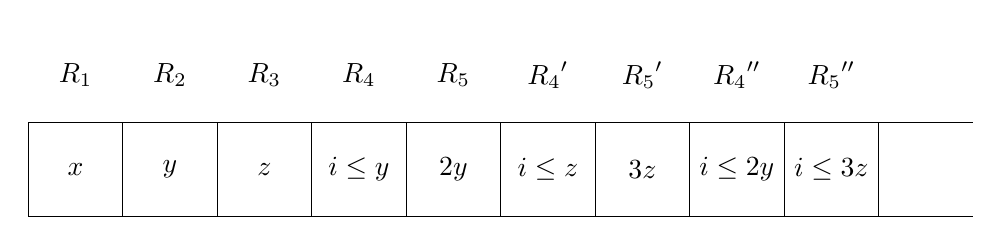
\begin{tikzpicture}[every node/.style={block},
        block/.style={minimum height=1.2cm,minimum width=1.2cm,outer sep=0pt,draw,rectangle,node distance=0pt}]
        
\node (b1) [label={$R_1$}] {$x$};
\node (b2) [right=of b1, label={$R_2$}] {$y$};
\node (b3) [right=of b2, label={$R_3$}] {$z$};
\node (b4) [right=of b3, label={$R_4$}] {$i \leq y$};
\node (b5) [right=of b4, label={$R_5$}] {$2y$};
\node (b6) [right=of b5, label={${R_4}'$}] {$i \leq z$};
\node (b7) [right=of b6, label={${R_5}'$}] {$3z$};
\node (b8) [right=of b7, label={${R_4}''$}] {$i \leq 2y$};
\node (b9) [right=of b8, label={${R_5}''$}] {$i \leq 3z$};

\draw (b9.north east) -- ++(1.2cm,0)
	(b9.south east) -- ++(1.2cm,0);

\end{tikzpicture}

\newpage

Schemat blokowy:

\vspace{18pt}

\begin{center}

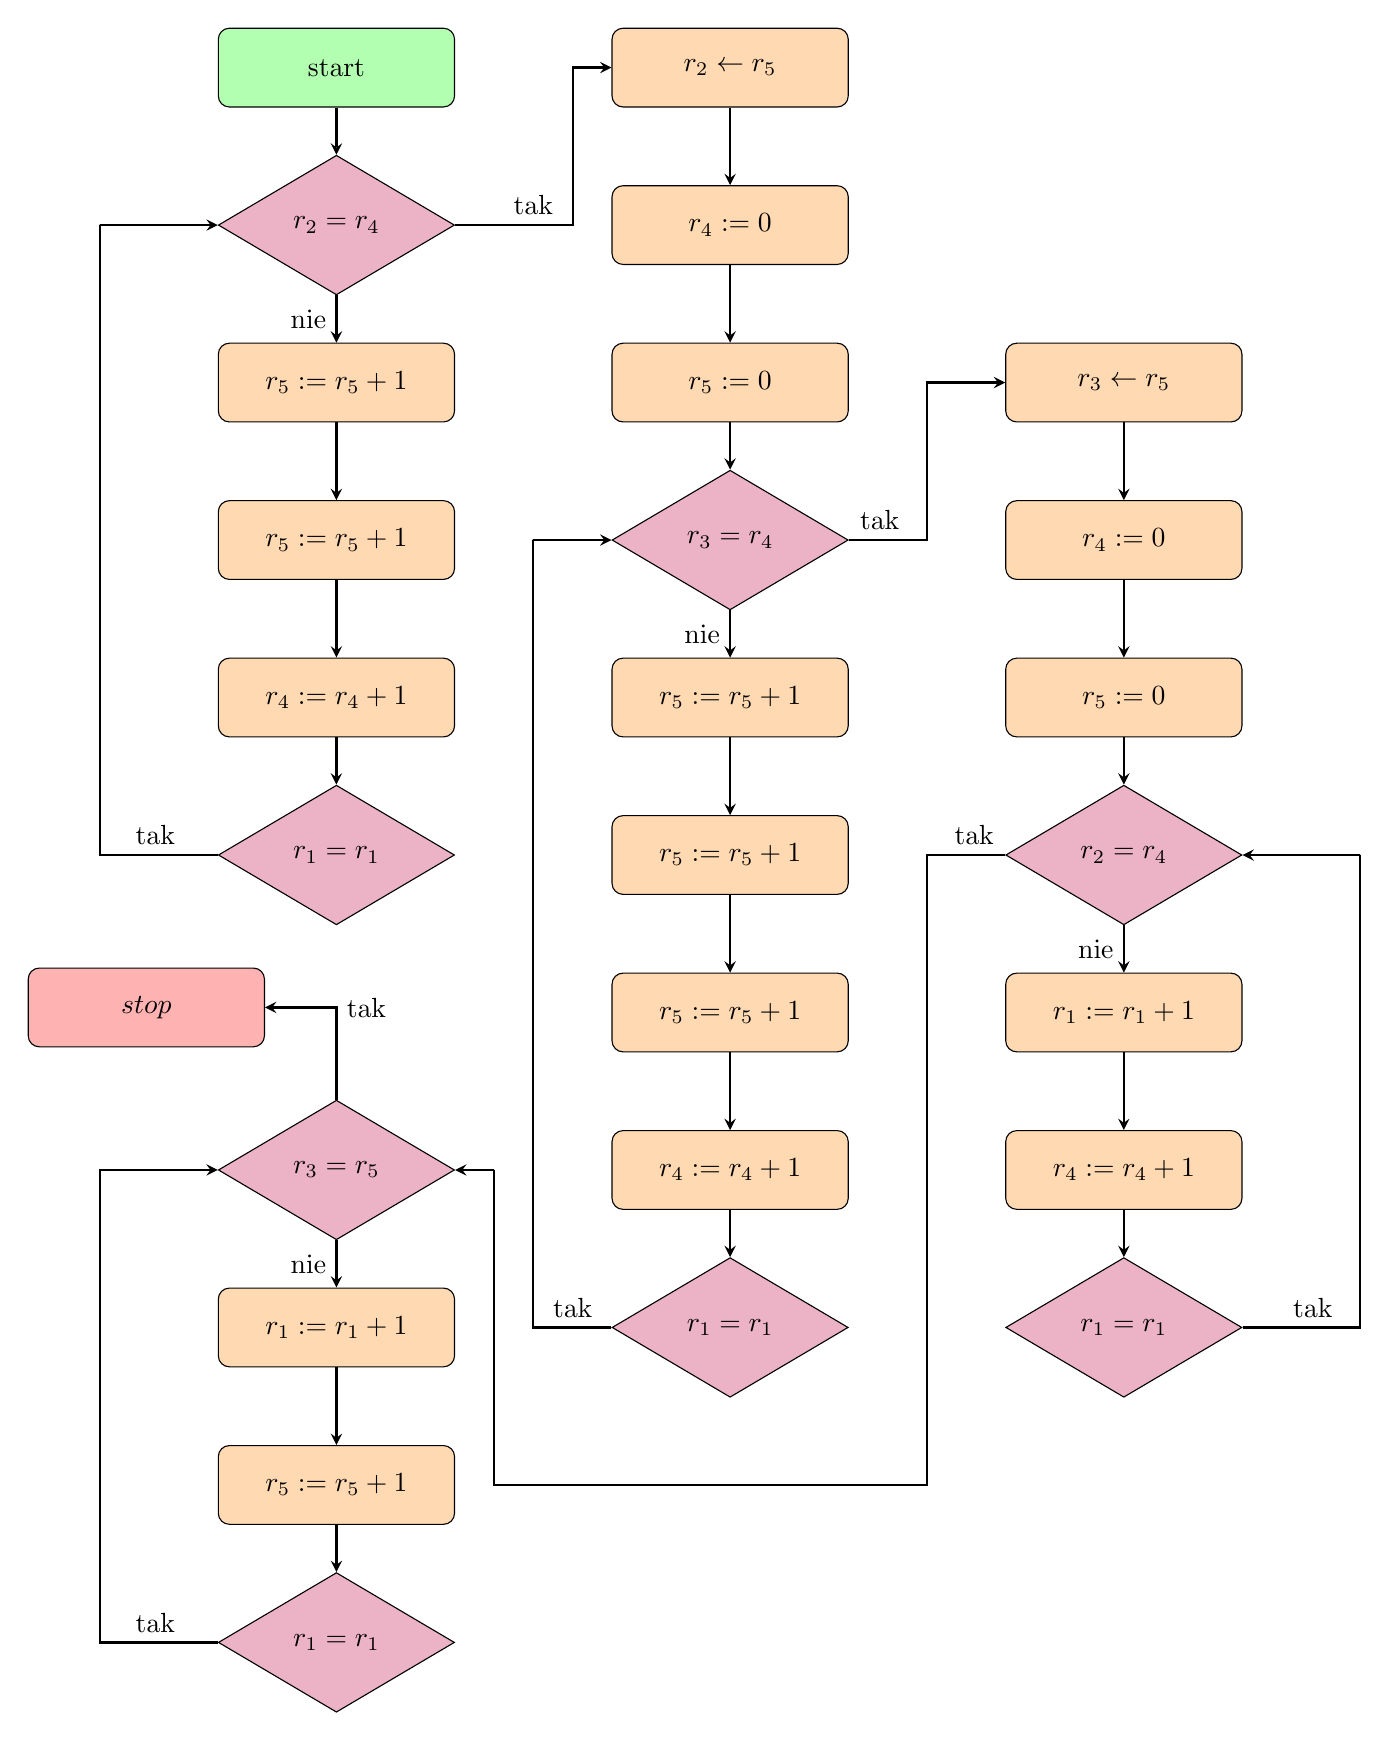
\begin{tikzpicture}[node distance=2cm]

\node (start) [start] {start};
\node (dec1) [decision, below of=start] {$r_2 = r_4$};
\node (inst1) [inst, below of=dec1] {$r_5:=r_5 + 1$};
\node (inst2) [inst, below of=inst1] {$r_5:=r_5 + 1$};
\node (inst3) [inst, below of=inst2] {$r_4:=r_4 + 1$};
\node (dec2) [decision, below of=inst3] {$r_1 = r_1$};

\node (inst4) [inst, right of=start,xshift=3cm] {$r_2 \leftarrow r_5$};
\node (inst5) [inst, below of=inst4] {$r_4:=0$};
\node (inst6) [inst, below of=inst5] {$r_5:=0$};
\node (dec3) [decision, below of=inst6] {$r_3=r_4$};
\node (inst7) [inst, below of=dec3] {$r_5:=r_5 + 1$};
\node (inst8) [inst, below of=inst7] {$r_5:=r_5 + 1$};
\node (inst9) [inst, below of=inst8] {$r_5:=r_5 + 1$};
\node (inst10) [inst, below of=inst9] {$r_4:=r_4 + 1$};
\node (dec4) [decision, below of=inst10] {$r_1=r_1$};

\node (inst11) [inst, right of=inst6, xshift=3cm] {$r_3 \leftarrow r_5$};
\node (inst12) [inst, below of=inst11] {$r_4:=0$};
\node (inst13) [inst, below of=inst12] {$r_5:=0$};
\node (dec5) [decision, below of=inst13] {$r_2=r_4$};
\node (inst14) [inst, below of=dec5] {$r_1:=r_1 + 1$};
\node (inst15) [inst, below of=inst14] {$r_4:=r_4+1$};
\node (dec6) [decision, below of=inst15] {$r_1=r_1$};

\node (dec7) [decision, left of=inst10, xshift=-3cm] {$r_3=r_5$};
\node (inst16) [inst, below of=dec7] {$r_1:=r_1 + 1$};
\node (inst17) [inst, below of=inst16] {$r_5:=r_5+1$};
\node (dec8) [decision, below of=inst17] {$r_1=r_1$};
\node (stop) [stop, above left of=dec7,xshift=-1cm,yshift=0.65cm] {$stop$};

\draw [arrow] (dec5) -| node[anchor=south,xshift=0.6cm]{tak}(7.5,-18) -| (2,-14) |- (dec7);
\draw [arrow] (start) -- (dec1);
\draw [arrow] (dec1) -- node[anchor=east]{nie}(inst1);
\draw [arrow] (inst1) -- (inst2);
\draw [arrow] (inst2) -- (inst3);
\draw [arrow] (inst3) -- (dec2);
\draw [arrow] (dec2) -| node[anchor=south,xshift=0.7cm]{tak} (-3,-2) |- (dec1);
\draw [arrow] (dec1) -| node[anchor=south,xshift=-0.5cm]{tak}(3,0) |- (inst4);
\draw [arrow] (inst4) -- (inst5);
\draw [arrow] (inst5) -- (inst6);
\draw [arrow] (inst6) -- (dec3);
\draw [arrow] (dec3) --  node[anchor=east]{nie}(inst7);
\draw [arrow] (inst7) -- (inst8);
\draw [arrow] (inst8) -- (inst9);
\draw [arrow] (inst9) -- (inst10);
\draw [arrow] (inst10) -- (dec4);
\draw [arrow] (dec4) -| node[anchor=south,xshift=0.5cm]{tak} (2.5,-6) |- (dec3);
\draw [arrow] (dec3) -| node[anchor=south,xshift=-0.6cm]{tak}(7.5,-5) |- (inst11);
\draw [arrow] (inst11) -- (inst12);
\draw [arrow] (inst12) -- (inst13);
\draw [arrow] (inst13) -- (dec5);
\draw [arrow] (dec5) -- node[anchor=east]{nie}(inst14);
\draw [arrow] (inst14) -- (inst15);
\draw [arrow] (inst15) -- (dec6);
\draw [arrow] (dec6) -| node[anchor=south,xshift=-0.6cm]{tak}(13,-10) |- (dec5);
\draw [arrow] (dec7) -- node[anchor=east]{nie}(inst16);
\draw [arrow] (inst16) -- (inst17);
\draw [arrow] (inst17) -- (dec8);
\draw [arrow] (dec8)  -| node[anchor=south,xshift=0.7cm]{tak} (-3,-15) |- (dec7);
\draw [arrow] (dec7) |- node[anchor=west]{tak}(stop);

\end{tikzpicture}

\end{center}

\newpage

\noindent\textbf{Zad 1.18.} Czy funkcja
\[ f(x,y,z) = 
  \begin{cases}
   	x + y - z, & \text{jeżeli } x + y \geq z, \\
   	\uparrow, & \text{w przeciwnym przypadku.} 
  \end{cases}
\]
jest  URM–obliczalna?  Jeżeli  tak  to  napisz  program.  W  tym  przypadku  narysuj typowe konfiguracje obliczeniowe (z odpowiednimi zmiennymi). Narysuj schemat blokowy programu.

Rozwiązanie.

\vspace{5pt}

Program:

\vspace{5pt}

\begin{Parallel}{0.1\textwidth}{0.55\textwidth}

\ParallelLText{
\hspace{160pt} $I_1$ 
\par
\hspace{160pt}  $I_2$ 
\par
\hspace{160pt}  $I_3$ 
\par
\hspace{160pt}  $I_4$ 
\par
\hspace{160pt}  $I_5$ 
\par 
\hspace{160pt}  $I_6$ 
\par 
\hspace{160pt}  $I_7$ 
\par 
\hspace{160pt} $I_8$ 
\par
\hspace{160pt} $I_9$ 
\par
\hspace{160pt}  $I_{10}$ 
}

\ParallelRText{
$J(2,4,5)$

$S(1)$

$S(4)$

$J(1,1,1)$

$T(3,4)$

$J(1,4,10)$

$S(5)$

$S(4)$

$J(1,1,6)$

$T(5,1)$
}

\end{Parallel}

\vspace{10pt}

Typowa konfiguracja:

\vspace{5pt}

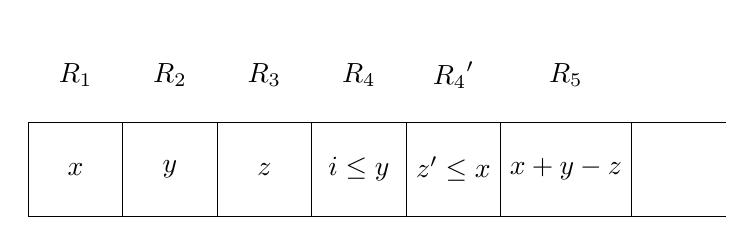
\begin{tikzpicture}[every node/.style={block},
        block/.style={minimum height=1.2cm,minimum width=1.2cm,outer sep=0pt,draw,rectangle,node distance=0pt}]
        
\node (b1) [label={$R_1$}] {$x$};
\node (b2) [right=of b1, label={$R_2$}] {$y$};
\node (b3) [right=of b2, label={$R_3$}] {$z$};
\node (b4) [right=of b3, label={$R_4$}] {$i \leq y$};
\node (b5) [right=of b4, label={${R_4}'$}] {$z' \leq x$};
\node (b6) [right=of b5, label={$R_5$}] {$x+y-z$};

\draw (b6.north east) -- ++(1.2cm,0)
	(b6.south east) -- ++(1.2cm,0);

\end{tikzpicture}


\newpage

Schemat blokowy:

\vspace{100pt}

\begin{center}

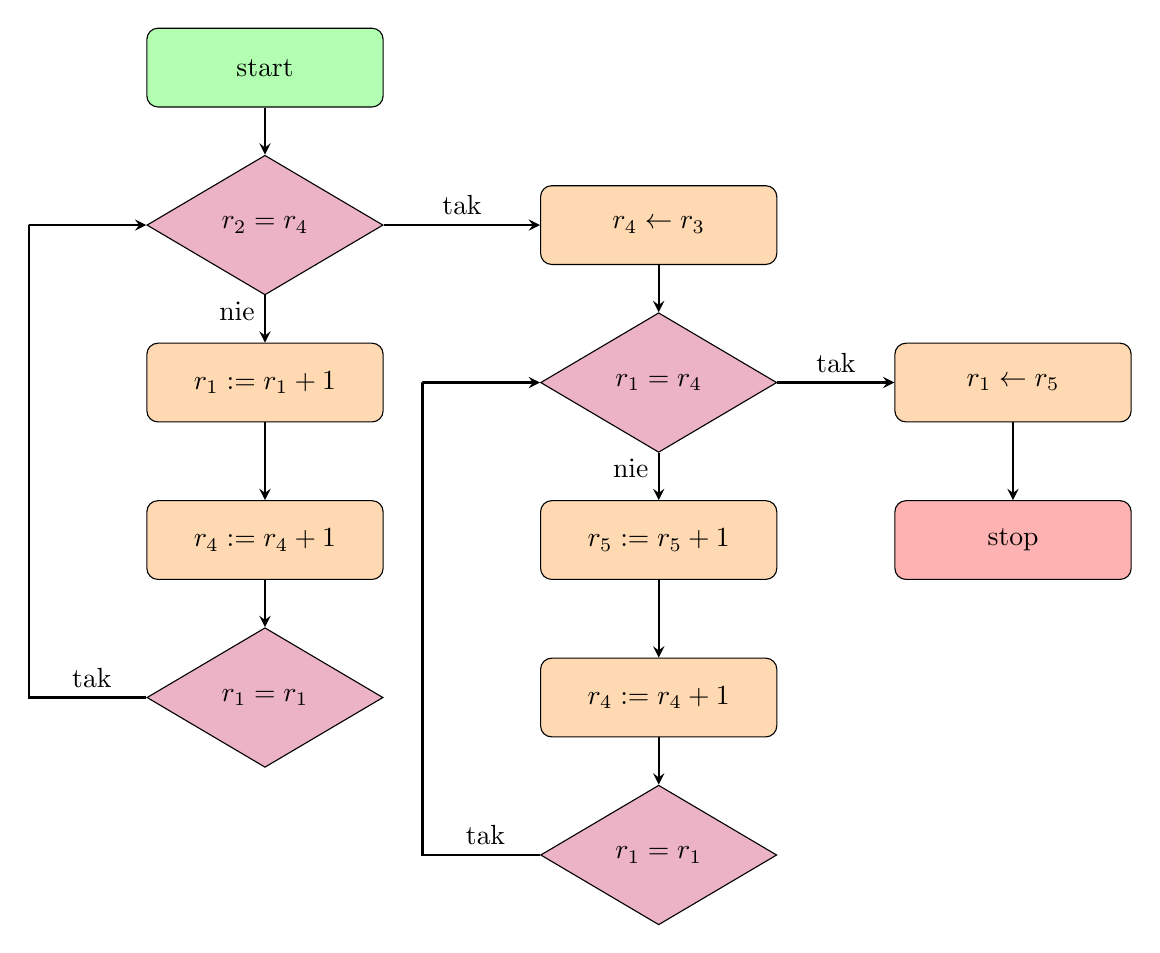
\begin{tikzpicture}[node distance=2cm]

\node (start) [start] {start};
\node (dec1) [decision, below of=start] {$r_2 = r_4$};
\node (inst1) [inst, below of=dec1] {$r_1:=r_1 + 1$};
\node (inst2) [inst, below of=inst1] {$r_4:=r_4 + 1$};
\node (dec2) [decision, below of=inst2] {$r_1 = r_1$};
\node (inst3) [inst, right of=dec1, xshift=3cm] {$r_4 \leftarrow  r_3$};
\node (dec3) [decision, below of=inst3] {$r_1 = r_4$};
\node (inst4) [inst, below of=dec3] {$r_5:=r_5 + 1$};
\node (inst5) [inst, below of=inst4] {$r_4:=r_4 + 1$};
\node (dec4) [decision, below of=inst5] {$r_1 = r_1$};
\node (inst6) [inst, right of=dec3, xshift=2.5cm] {$r_1 \leftarrow  r_5$}; 
\node (stop) [stop, below of=inst6] {stop}; 
 
\draw [arrow] (dec2) -| node[anchor=south,xshift=0.8cm]{tak}(-3,-2) |- (dec1);
\draw [arrow] (start) -- (dec1);
\draw [arrow] (dec1) -- node[anchor=east,yshift=0.1cm]{nie}(inst1);
\draw [arrow] (inst1) -- (inst2);
\draw [arrow] (inst2) -- (dec2);
\draw [arrow] (dec1) -- node[anchor=south]{tak}(inst3);
\draw [arrow] (inst3) -- (dec3);
\draw [arrow] (dec3) -- node[anchor=east,yshift=0.1cm]{nie}(inst4);
\draw [arrow] (inst4) -- (inst5);
\draw [arrow] (inst5) -- (dec4);
\draw [arrow] (dec4) -| node[anchor=south,xshift=0.8cm]{tak}(2,-4) |- (dec3);
\draw [arrow] (dec3) -- node[anchor=south]{tak}(inst6);
\draw [arrow] (inst6) -- (stop);

\end{tikzpicture}

\end{center}

\newpage

\noindent\textbf{Zad 1.20.} Czy funkcja
\[ f(x,y,z) = 
  \begin{cases}
   	z + \frac{1}{2}(x - y), & \text{jeżeli } x \geq y \text{ i x - y jest parzyste}, \\
   	\uparrow, & \text{w przeciwnym przypadku.} 
  \end{cases}
\]
jest  URM–obliczalna?  Jeżeli  tak  to  napisz  program.  W  tym  przypadku  narysuj typowe konfiguracje obliczeniowe (z odpowiednimi zmiennymi). Narysuj schemat blokowy programu.

Rozwiązanie.

\vspace{5pt}

Program:

\vspace{5pt}

\begin{Parallel}{0.1\textwidth}{0.55\textwidth}

\ParallelLText{
\hspace{160pt} $I_1$ 
\par
\hspace{160pt}  $I_2$ 
\par
\hspace{160pt}  $I_3$ 
\par
\hspace{160pt}  $I_4$ 
\par
\hspace{160pt}  $I_5$ 
\par 
\hspace{160pt}  $I_6$ 
\par 
\hspace{160pt}  $I_7$ 
\par 
\hspace{160pt} $I_8$ 
\par
\hspace{160pt} $I_9$ 
\par
\hspace{160pt}  $I_{10}$ 
\par
\hspace{160pt}  $I_{11}$ 
\par 
\hspace{160pt}  $I_{12}$ 
\par 
\hspace{160pt}  $I_{13}$ 
\par 
\hspace{160pt} $I_{14}$ 
\par
\hspace{160pt} $I_{15}$ 
\par
\hspace{160pt} $I_{16}$ 
\par
\hspace{160pt} $I_{17}$ 
\par 
\hspace{160pt} $I_{18}$ 
\par 
\hspace{160pt} $I_{19}$  
}

\ParallelRText{
$J(2,6,5)$

$S(5)$

$S(6)$

$J(1,1,1)$

$J(1,5,9)$

$S(4)$

$S(5)$

$J(1,1,5)$

$T(4,1)$

$J(1,7,15)$

$S(7)$

$S(7)$

$S(8)$

$J(1,1,10)$

$T(8,1)$

$J(3,9,20)$

$S(1)$

$S(9)$

$J(1,1,16)$
}

\end{Parallel}

\vspace{10pt}

Typowa konfiguracja:

\vspace{5pt}

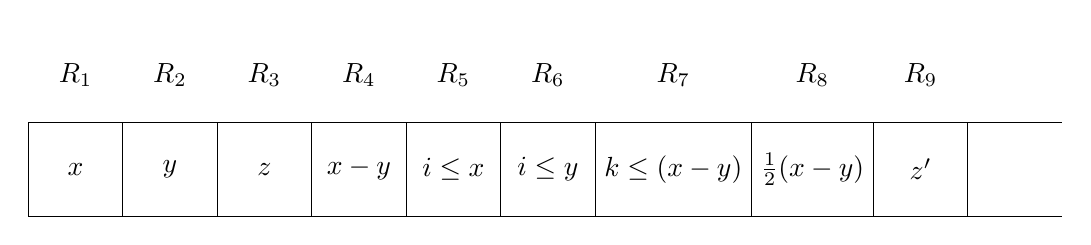
\begin{tikzpicture}[every node/.style={block},
        block/.style={minimum height=1.2cm,minimum width=1.2cm,outer sep=0pt,draw,rectangle,node distance=0pt}]
        
\node (b1) [label={$R_1$}] {$x$};
\node (b2) [right=of b1, label={$R_2$}] {$y$};
\node (b3) [right=of b2, label={$R_3$}] {$z$};
\node (b4) [right=of b3, label={$R_4$}] {$x-y$};
\node (b5) [right=of b4, label={$R_5$}] {$i \leq x$};
\node (b6) [right=of b5, label={$R_6$}] {$i \leq y$};
\node (b7) [right=of b6, label={$R_7$}] {$k \leq (x-y)$};
\node (b8) [right=of b7, label={$R_8$}] {$\frac{1}{2}(x-y)$};
\node (b9) [right=of b8, label={$R_9$}] {$z'$};

\draw (b9.north east) -- ++(1.2cm,0)
	(b9.south east) -- ++(1.2cm,0);

\end{tikzpicture}

\newpage

Schemat blokowy:

\vspace{25pt}

\begin{tikzpicture}[node distance=2cm]

\node (start) [start] {start};
\node (dec1) [decision, below of=start] {$r_2 = r_6$};
\node (inst1) [inst, below of=dec1] {$r_5:=r_5 + 1$};
\node (inst2) [inst, below of=inst1] {$r_6:=r_6 + 1$};
\node (dec2) [decision, below of=inst2] {$r_1 = r_1$};
\node (dec5) [decision, right of=dec1, xshift=3cm] {$r_1 = r_5$};
\node (inst4) [inst, below of=dec5] {$r_4:=r_4 + 1$};
\node (inst5) [inst, below of=inst4] {$r_5:=r_5 + 1$};
\node (dec4) [decision, below of=inst5] {$r_1 = r_1$};
\node (inst6) [inst, right of=dec5, xshift=2.5cm] {$r_1 \leftarrow  r_4$}; 
\node (dec6) [decision, below of=inst6] {$r_1 = r_7$};
\node (inst7) [inst, below of=dec6] {$r_7:=r_7 + 1$};
\node (inst8) [inst, below of=inst7] {$r_7:=r_7 + 1$};
\node (inst9) [inst, below of=inst8] {$r_8:=r_8 + 1$};
\node (dec7) [decision, below of=inst9] {$r_1 = r_1$};
\node (inst10) [inst, left of=dec7,xshift=-3cm] {$r_1 \leftarrow r_8$};
\node (dec8) [decision, below of=inst10]{$r_3 = r_9$};
\node (inst11) [inst, below of=dec8] {$r_1: =r_1 + 1$};
\node (inst12) [inst, below of=inst11] {$r_9: =r_9 + 1$};
\node (dec9) [decision, below of=inst12]{$r_1 = r_1$};
\node (stop) [stop, right of=dec8,xshift=3cm] {$stop$};
 
\draw [arrow] (dec2) -| node[anchor=south,xshift=0.8cm]{tak}(-3,-2) |- (dec1);
\draw [arrow] (start) -- (dec1);
\draw [arrow] (dec1) -- node[anchor=east,yshift=0.1cm]{nie}(inst1);
\draw [arrow] (inst1) -- (inst2);
\draw [arrow] (inst2) -- (dec2);
\draw [arrow] (dec1) -- node[anchor=south]{tak}(inst3);
\draw [arrow] (dec5) -- node[anchor=east,yshift=0.1cm]{nie}(inst4);
\draw [arrow] (inst4) -- (inst5);
\draw [arrow] (inst5) -- (dec4);
\draw [arrow] (dec5) -- node[anchor=south]{tak}(inst6);
\draw [arrow] (dec4) -|node[anchor=south,xshift=0.5cm]{tak} (2.5, -2) |- (dec5);
\draw [arrow] (inst6) -- (dec6);
\draw [arrow] (dec6) -- node[anchor=east,yshift=0.1cm]{nie}(inst7);
\draw [arrow] (inst7) -- (inst8);
\draw [arrow] (inst8) -- (inst9);
\draw [arrow] (inst9) -- (dec7);
\draw [arrow] (dec7) -| node[anchor=south,xshift=-0.8cm]{tak}(13,-4) |- (dec6);
\draw [arrow] (dec6) -| node[anchor=south,xshift=0.5cm]{tak}(7, -4) |- (inst10);
\draw [arrow] (inst10) -- (dec8);
\draw [arrow] (dec8) -- node[anchor=east,yshift=0.1cm]{nie}(inst11);
\draw [arrow] (inst11) -- (inst12);
\draw [arrow] (inst12) -- (dec9);
\draw [arrow] (dec8) -- node[anchor=south]{tak}(stop);
\draw [arrow] (dec9) -| node[anchor=south,xshift=0.5cm]{tak}(2.0, -14) |- (dec8);

\end{tikzpicture}

\newpage

\noindent\textbf{Zad 1.22.} Niech program P będzie dany przez

\vspace{10pt}

\begin{Parallel}{0.1\textwidth}{0.55\textwidth}

\ParallelLText{
\hspace{160pt} $I_1$ 
\par
\hspace{160pt}  $I_2$ 
\par
\hspace{160pt}  $I_3$ 
\par
\hspace{160pt}  $I_4$ 
\par
\hspace{160pt}  $I_5$ 
\par 
\hspace{160pt}  $I_6$ 
\par 
\hspace{160pt}  $I_7$ 
}

\ParallelRText{
$J(1,4,9)$

$S(3)$

$J(1,3,7)$

$S(2)$

$S(3)$

$J(1,1,3)$

$T(2,1)$
}

\end{Parallel}

\vspace{10pt}

Jaka jednoargumentowa funkcja zmiennej n jest obliczana przez ten program? Narysuj schemat blokowy programu P. Obowiązkowo narysuj typowe konfiguracje obliczeniowe (z odpowiednimi zmiennymi). 

Rozwiązanie.

\vspace{5pt}

Funkcja f(n) obliczana przez program to:
\[ f(n) = 
  \begin{cases}
  	0, & \text{jeżeli } n = 0, \\
  	n - 1, & \text{jeżeli } n \geq 1 
  \end{cases}
\]

\vspace{5pt}

Typowa konfiguracja:

\vspace{5pt}

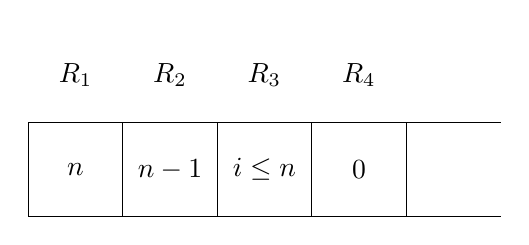
\begin{tikzpicture}[every node/.style={block},
        block/.style={minimum height=1.2cm,minimum width=1.2cm,outer sep=0pt,draw,rectangle,node distance=0pt}]
        
\node (b1) [label={$R_1$}] {$n$};
\node (b2) [right=of b1, label={$R_2$}] {$n-1$};
\node (b3) [right=of b2, label={$R_3$}] {$i \leq n$};
\node (b4) [right=of b3, label={$R_4$}] {$0$};

\draw (b4.north east) -- ++(1.2cm,0)
	(b4.south east) -- ++(1.2cm,0);

\end{tikzpicture}

\newpage

Schemat blokowy:

\vspace{90pt}

\begin{center}

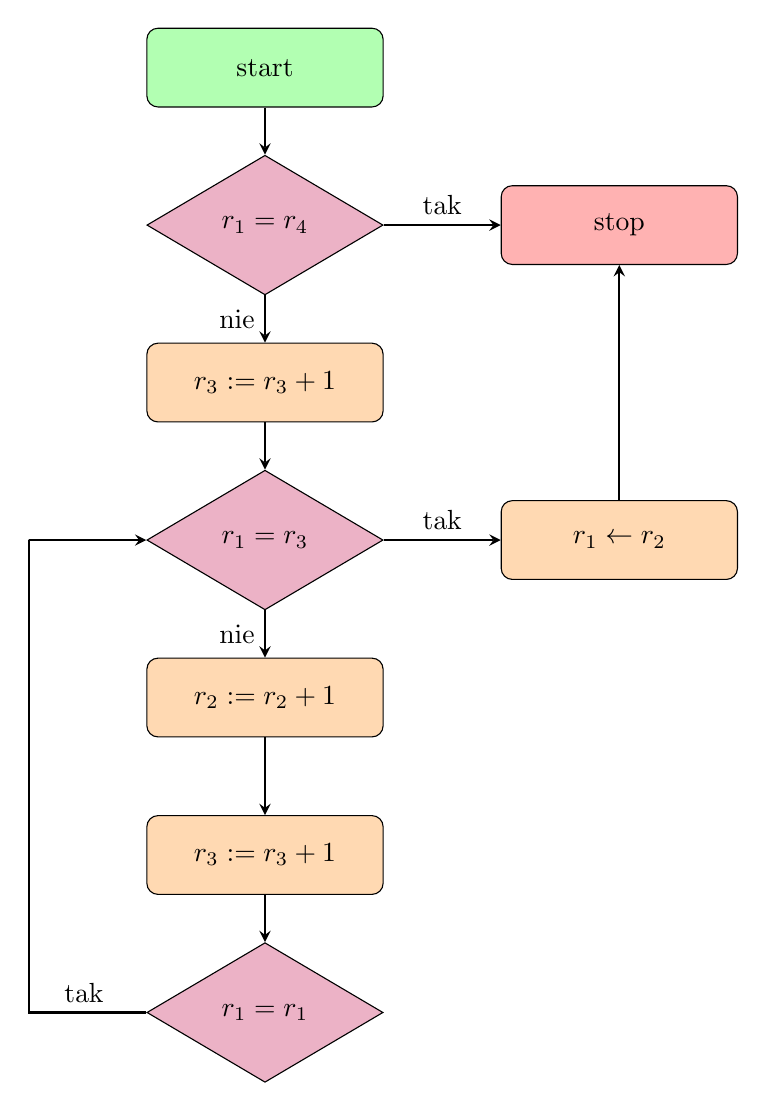
\begin{tikzpicture}[node distance=2cm]

\node (start) [start] {start};
\node (dec1) [decision, below of=start] {$r_1 = r_4$};
\node (inst1) [inst,below of=dec1]{$r_3:=r_3 + 1$};
\node (dec2) [decision, below of=inst1] {$r_1 = r_3$};
\node (inst2) [inst,below of=dec2]{$r_2:=r_2 + 1$};
\node (inst3) [inst,below of=inst2]{$r_3:=r_3 + 1$};
\node (dec3) [decision, below of=inst3] {$r_1 = r_1$};
\node (stop) [stop, right of=dec1, xshift=2.5cm] {stop};
\node (inst4) [inst,right of=dec2, xshift=2.5cm]{$r_1 \leftarrow r_2$};

\draw [arrow] (start) -- (dec1);
\draw [arrow] (dec1) -- node[anchor=south]{tak}(stop);
\draw [arrow] (dec1) -- node[anchor=east]{nie}(inst1);
\draw [arrow] (inst1) -- (dec2);
\draw [arrow] (dec2) -- node[anchor=south]{tak}(inst4);
\draw [arrow] (inst4) -- (stop);
\draw [arrow] (dec2) -- node[anchor=east]{nie}(inst2);
\draw [arrow] (inst2) -- (inst3);
\draw [arrow] (inst3) -- (dec3);
\draw [arrow] (dec3) -|node[anchor=south,xshift=0.7cm]{tak} (-3,-6) |- (dec2);

\end{tikzpicture}

\end{center}

\end{document}